\documentclass[../main.tex]{subfiles}
\graphicspath{{\subfix{../Images/}}}
\begin{document}
\section{Functions}

\subsection{Set Notation}
\begin{tabular}{|c|c|c|}
    \hline
    \textbf{Symbol} & \textbf{Meaning} & \textbf{Example} \\
    \hline
    \(\mathbb{N}\) & Natural Numbers & \(\{1,2,3, \cdots\}\) \\
    \hline
    \(\mathbb{Z}^{+}_{0}\) & Non -ve Integers & \(\{0,1,2, \cdots\}\) \\
    \hline
    \(\mathbb{Z}\) & Integers & \(\{\cdots ,-1,0,1, \cdots\}\) \\
    \hline
    \(\mathbb{Q}\) & Rationals & \(\{\frac{p}{q} : \, p,q \in \mathbb{Z}\}\) \\
    \hline
    \(\mathbb{R}\) & Real Numbers & \(\{\cdots, -\pi, \frac{1}{2}, \sqrt{2}, 2 \cdots\}\) \\
    \hline
    \(\mathbb{C}\) & Complex Numbers & \(\{a+bi : \, a,b \in \mathbb{R}\}\) \\
    \hline
\end{tabular} \\
\boxedeq{\mathbb{N} \subset \mathbb{Z}^{+}_{0} \subset \mathbb{Z} \subset \mathbb{Q} \subset \mathbb{R} \subset \mathbb{C}}

\subsubsection{Interval Notation}
\begin{tabular}{|c|c|}
    \hline
    \textbf{Notation} & \textbf{Definition} \\
    \hline
    \([a,b]\) & \(\{x\in\mathbb{R} : a \leq x \leq b\}\) \\
    \hline
    \((a,b)\) & \(\{x\in\mathbb{R} : a < x < b\}\) \\
    \hline
    \((a,b]\) & \(\{x\in\mathbb{R} : a < x \leq b\}\) \\
    \hline
    \((-\infty,b]\) & \(\{x\in\mathbb{R} : x \leq b\}\) \\
    \hline
    \([a,b) \cup (c,\infty)\) & \(\{x\in\mathbb{R} : a \leq x < b \text{ or } x > c\}\) \\
    \hline
    \([a,c) \cap [b,\infty)\) & \(\{x\in\mathbb{R} : b \leq x < c\}\) \\
    \hline
    \(\mathbb{R}\backslash\{0\}\) & \(\{x\in\mathbb{R} : x \neq 0\}\) \\
    \hline
\end{tabular} \\\\
\textbf{Notes} \\
Interval and Set Notations are not exact replacements \\* of each other even though they are similar

\subsection{Definitions}
\subsubsection{Notations}
\begin{tabular}{|c|c|}
    \hline
    \textbf{Representation} & \textbf{Meaning} \\
    \hline
    \(f\) & function \\
    \hline
    \(f:A \to B\) & Set Mapping \\
    \hline
    \(f:x \mapsto x^2\) & Rule of function \\
    \hline
    \(f(x)\) & Rule of function \\
    \hline
    \(D_{f}\) & Domain of \(f\) \\
    \hline
    \(R_{f}\) & Range of \(f\) \\
    \hline
\end{tabular}
\newpage \noindent

\subsubsection{Relations}
The Associatation between 2 Sets is a Relation \\
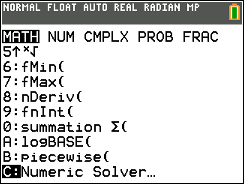
\includegraphics[scale=0.7]{2 Functions/Capture 1.png}

\subsubsection{Definition of a Function}
A \textbf{Function} is a relation from Set \(X\) to \(Y\) where every input \(x \in X\) is mapped to a \textbf{unique output} \(y \in Y\) \\\\
With this definition, we can see from 3.2.2 that only (a) \& (b) are functions.
(c) is not a function as input \((x=-1)\) is mapped to \(y=-1\) \& \(y=1\), (d) in
not a function as input \((x=5)\) does not have a related output in \(Y\) \\\\
%Function Notation%
Function Example:
\begin{align*}
    \displaystyle f:x \mapsto x, \, & x \in (-2,2) \\
        \text{Rule}\phantom{spa} & \phantom{s }\text{Domain}
\end{align*}

\subsubsection{Finding Range with GC}
Key the function into the GC, while taking note of the starting and ending points of the domain.
If the function has turning points, it has to be taken into account as it coul affect the Range. \\\\
Example: \\
\(\displaystyle f:x \mapsto e^{x^{2}+2x+1}\), \(x \in [-2,0.5)\) \\
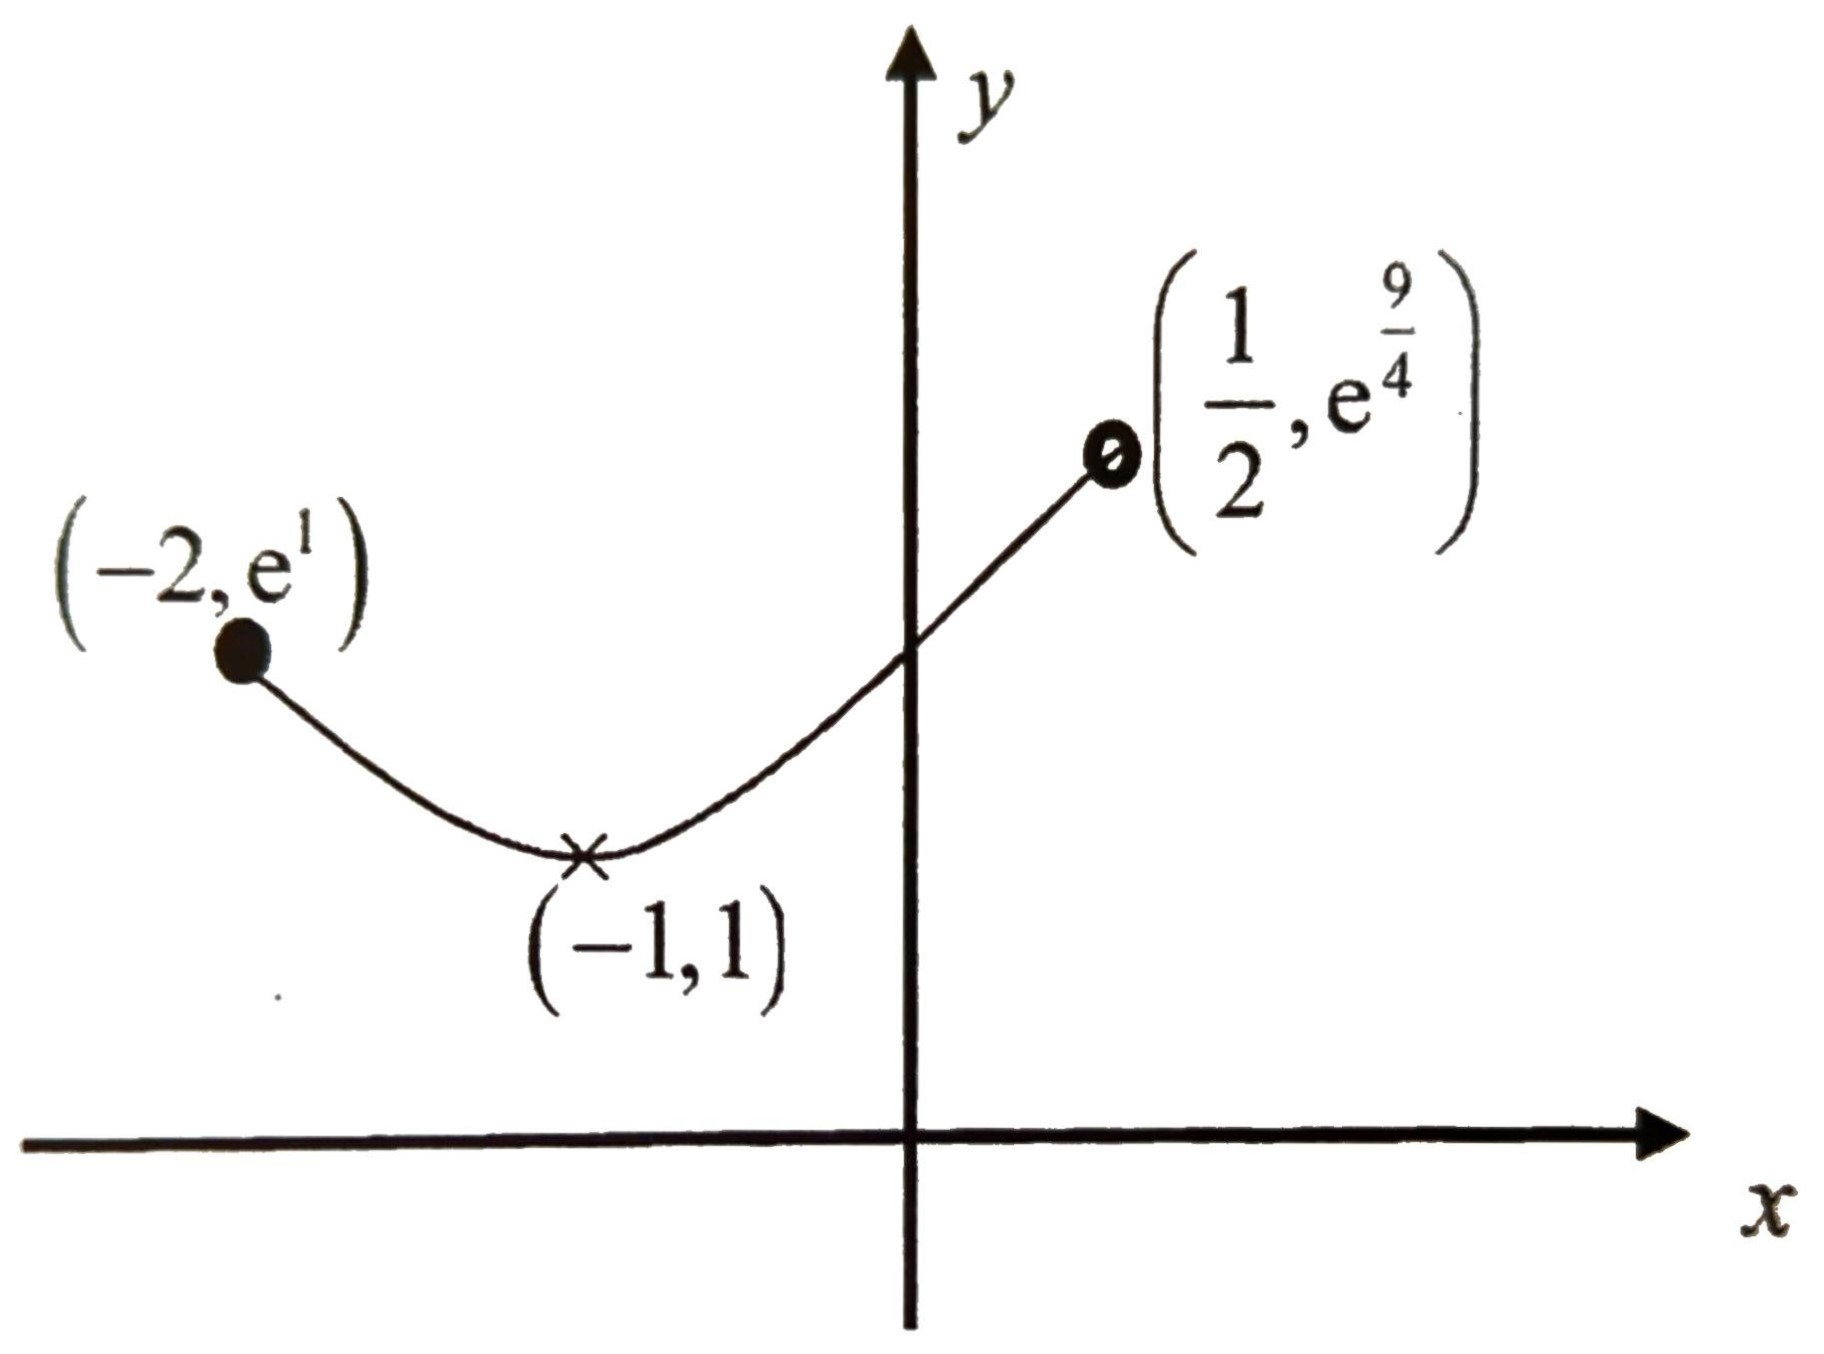
\includegraphics[scale=0.1]{2 Functions/Capture 2.jpg} \\
\(\therefore R_{f} = \left[1,e^{\textstyle \frac{9}{4}}\right)\)

\subsection{Injective Functions}

\subsubsection{Definition of Injection}

\subsubsection{Disproving Injectivity}

\subsubsection{Proving Injevtivity}

\subsection{*Surjective Functions}

\subsubsection{Definition of Surjection}

\subsubsection{Proving or Disproving Surjevtivity}

\subsection{*Bijective Functions}

\subsubsection{Definition of Bijection}

\subsection{Inverse Functions}

\subsubsection{Invese Function Notation}

\subsubsection{Conditions for an inverse to exist}

\subsubsection{Properties of Inverse Functions}

\subsubsection{Self-Inversing functions}

\subsection{Composite Functions}

\subsubsection{Composite Function Notation}

\subsubsection{Conditions for a composition to exist}

\subsubsection{Finding Domain \& Range of a Composition}

\subsection{Extensions}

\subsubsection{Properties of Functions}

\subsubsection{Inverse Trigonometic Functions}

\subsubsection{Monotonic Functions}

\subsubsection{*Floor and Ceiling Functions}

\subsubsection{*Continuity \& Discontinuity}


\end{document}